
%(BEGIN_QUESTION)
% Copyright 2014, Tony R. Kuphaldt, released under the Creative Commons Attribution License (v 1.0)
% This means you may do almost anything with this work of mine, so long as you give me proper credit

Which component, the resistor or the capacitor, will drop more voltage in this circuit?

$$\includegraphics[width=15.5cm]{i01039x01.eps}$$

Also, calculate the total impedance ($Z_{total}$) of this circuit, expressing it in both rectangular and polar forms.

\underbar{file i01039}
%(END_QUESTION)





%(BEGIN_ANSWER)

The resistor will drop more voltage.

\vskip 10pt

$Z_{total}$ (rectangular form) = 5100 $\Omega$ $-$ j4671 $\Omega$

\vskip 10pt

$Z_{total}$ (polar form) = 6916 $\Omega$ $\angle$ $-42.5^{o}$

%(END_ANSWER)





%(BEGIN_NOTES)

Ask your students how they were able to make the determination of greater voltage drop.  Which method yields the fastest solution (i.e. requires the fewest steps)?

%INDEX% Electronics review: AC reactance and impedance

%(END_NOTES)


